%----------------------------------------------------------------------------------------
%	Appendices
%----------------------------------------------------------------------------------------

\part{Appendices}

\chapter{Hardware Topologies}

Appendix A contains circuit diagrams relating to hardware sensing and processing topologies. All component designators are arbitrary except R1, R2, R3, and R4 which represent the four load cells. Further, + and - are the positive and negative relationship strain gauges inside the load cells.

\begin{figure}[!ht]
	\centering
	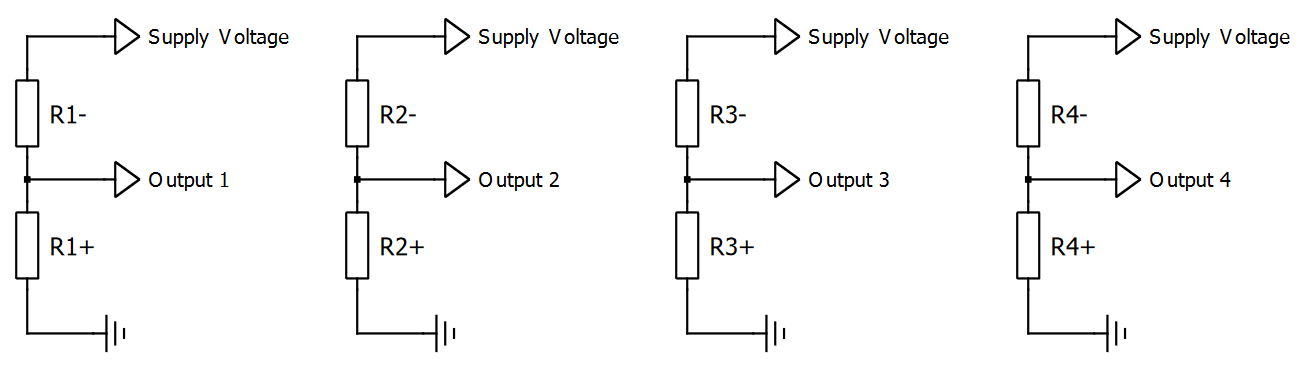
\includegraphics[scale=0.5]{hw-sensing-1.png}
	\caption{Individual load cell sensing topology.}
	\label{fig:sense-1}
\end{figure}

\begin{figure}[!ht]
	\centering
	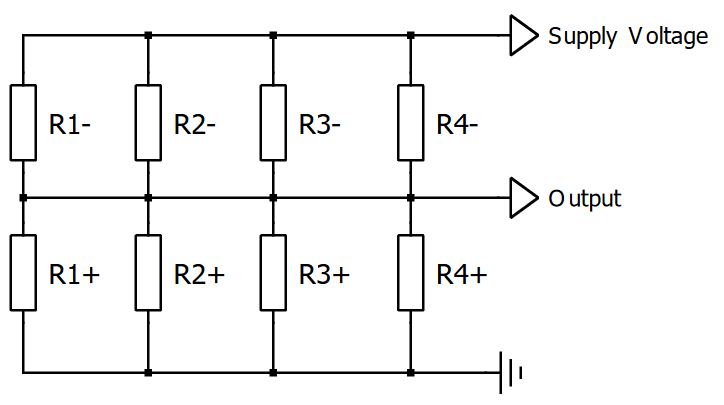
\includegraphics[scale=0.45]{hw-sensing-2.png}
	\caption{Parallel load cell sensing topology.}
	\label{fig:sense-2}
\end{figure}

\begin{figure}[!ht]
	\centering
	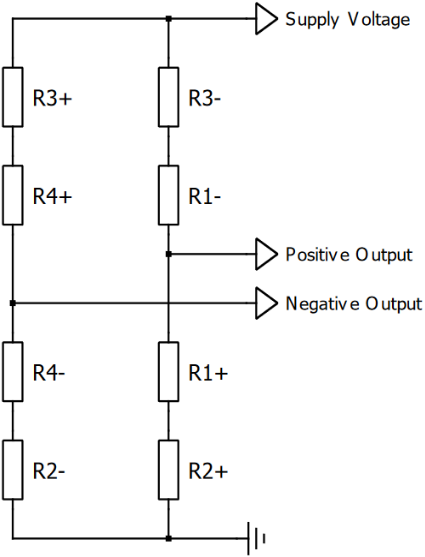
\includegraphics[scale=0.5]{hw-sensing-3.png}
	\caption{Wheatstone Bridge load cell sensing topology.}
	\label{fig:sense-3}
\end{figure}

\begin{figure}[!ht]
	\centering
	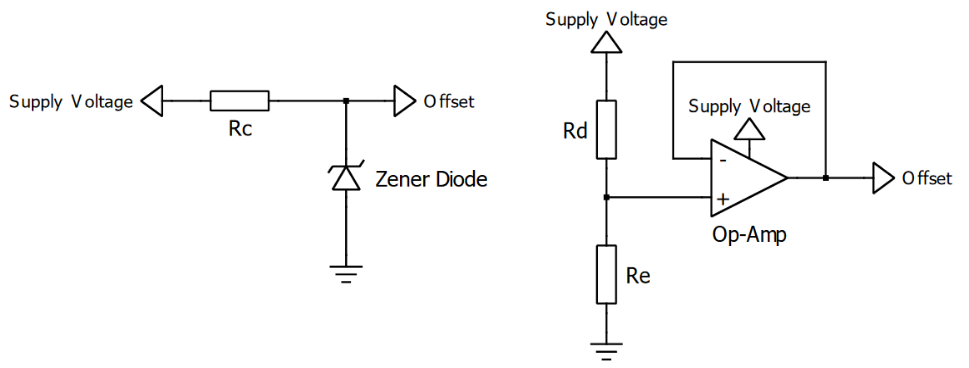
\includegraphics[scale=0.6]{hw-offset.png}
	\caption{a) Zener regulator b) Voltage divider with buffer.}
	\label{fig:offset}
\end{figure}

\begin{figure}[!ht]
	\centering
	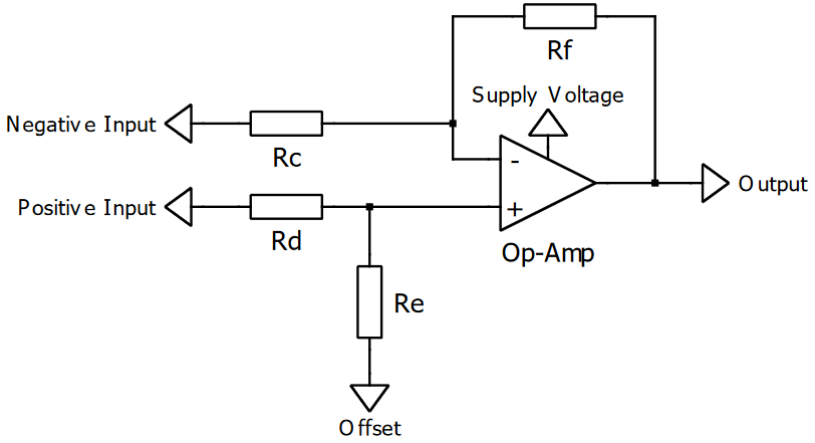
\includegraphics[scale=0.5]{hw-amplifier.png}
	\caption{Differential amplifier.}
	\label{fig:amplifier}
\end{figure}

\begin{figure}[!ht]
	\centering
	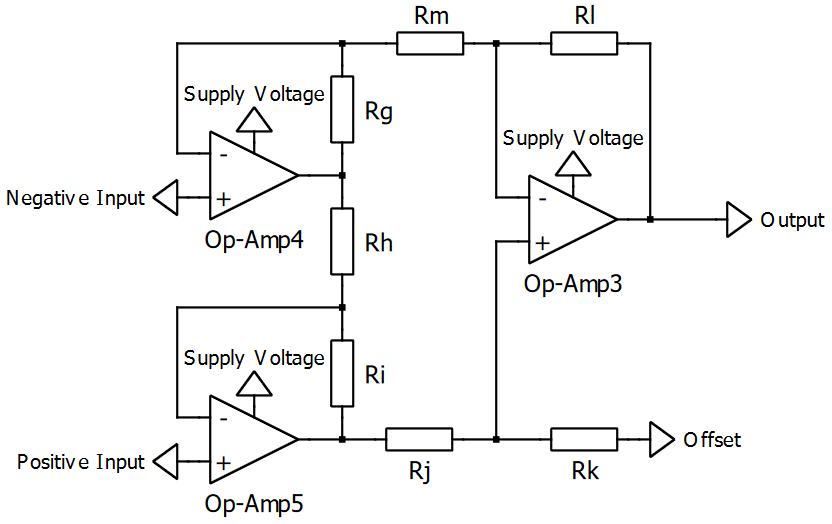
\includegraphics[scale=0.5]{hw-amplifier-1.png}
	\caption{Instrumentation amplifier.}
	\label{fig:amplifier-2}
\end{figure}

\chapter{Gantt Chart}

\begin{figure}[!ht]
	\centering
	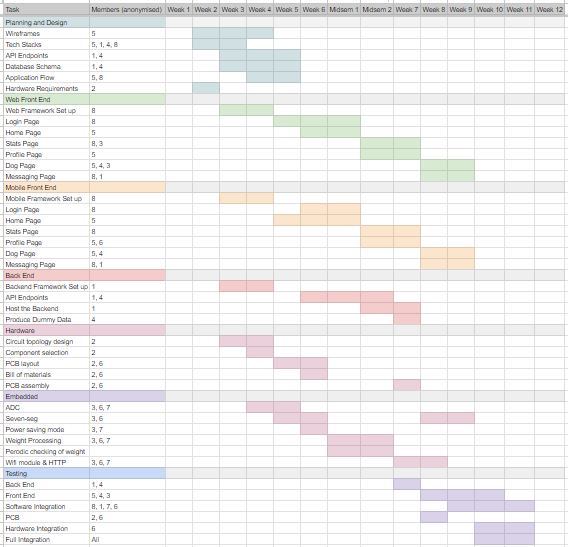
\includegraphics[scale=0.8]{gantt-chart.png}
	\caption{Gantt Chart.}
	\label{fig:gantt-chart-1}
\end{figure}

\chapter{Database Diagram}

\begin{figure}[!ht]
	\centering
	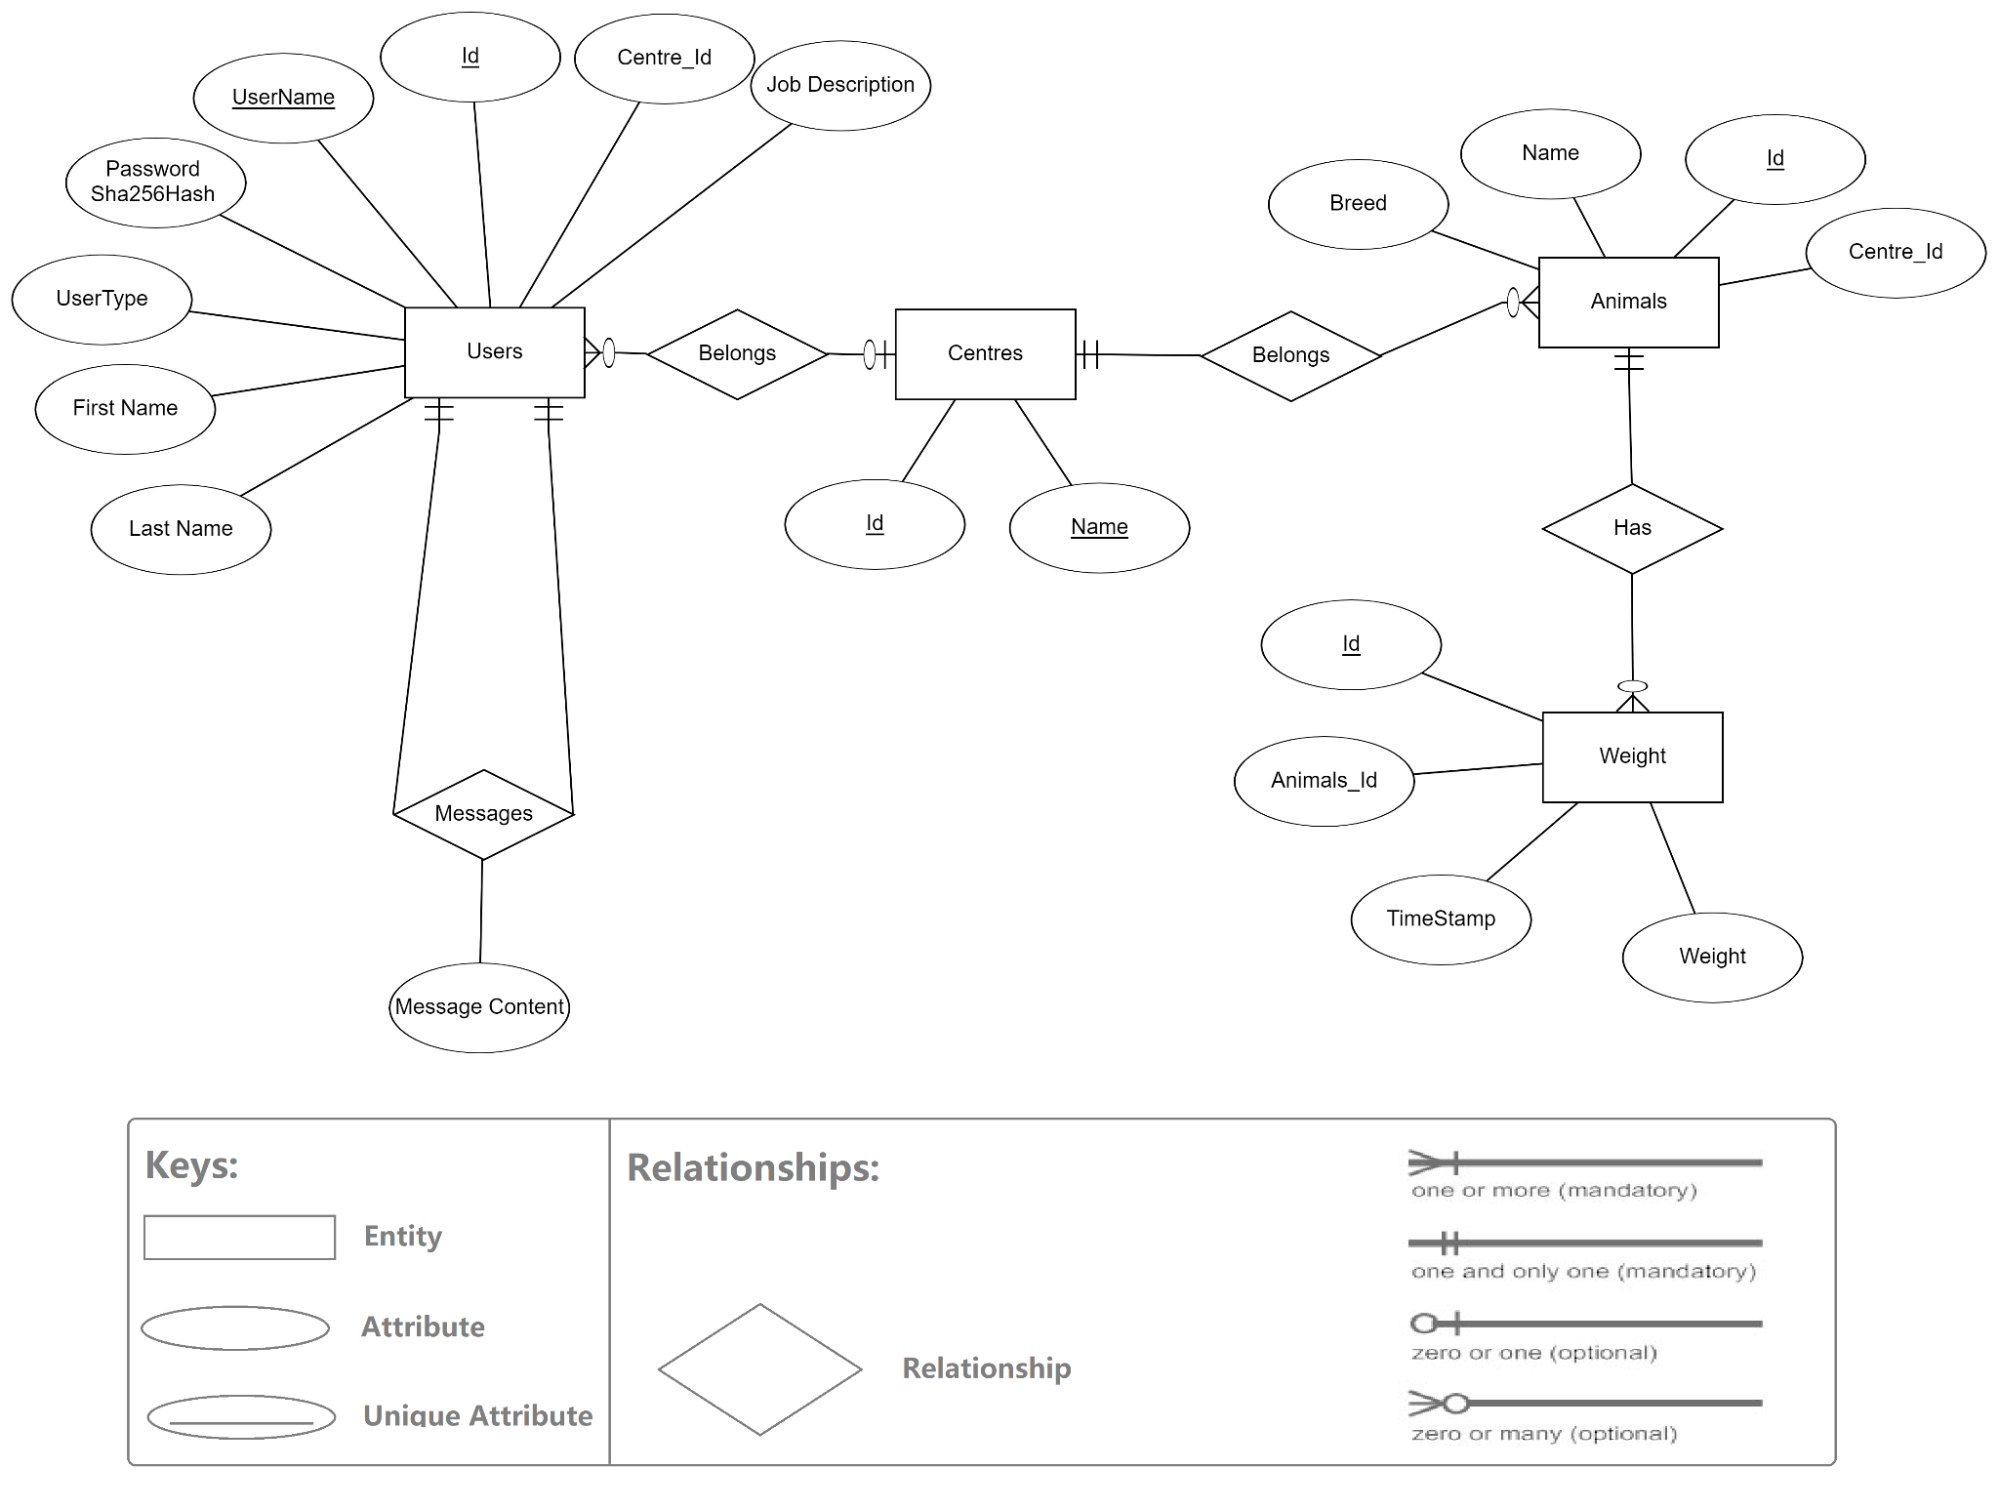
\includegraphics[scale=0.2]{sw-database.png}
	\caption{SQL Database Entity Relationship Diagram Draft.}
	\label{fig:database-1}
\end{figure}

\chapter{Frontend Software Wireframes}

Appendix D contains additional wireframes for the frontend. The full design can be found at https://www.figma.com/file/phTrRMMdn89c7amXQTm92d/770-design?node-id=0%3A1&t=FWLBtxPM2iXpupKZ-1

\begin{figure}[!ht]
	\centering
	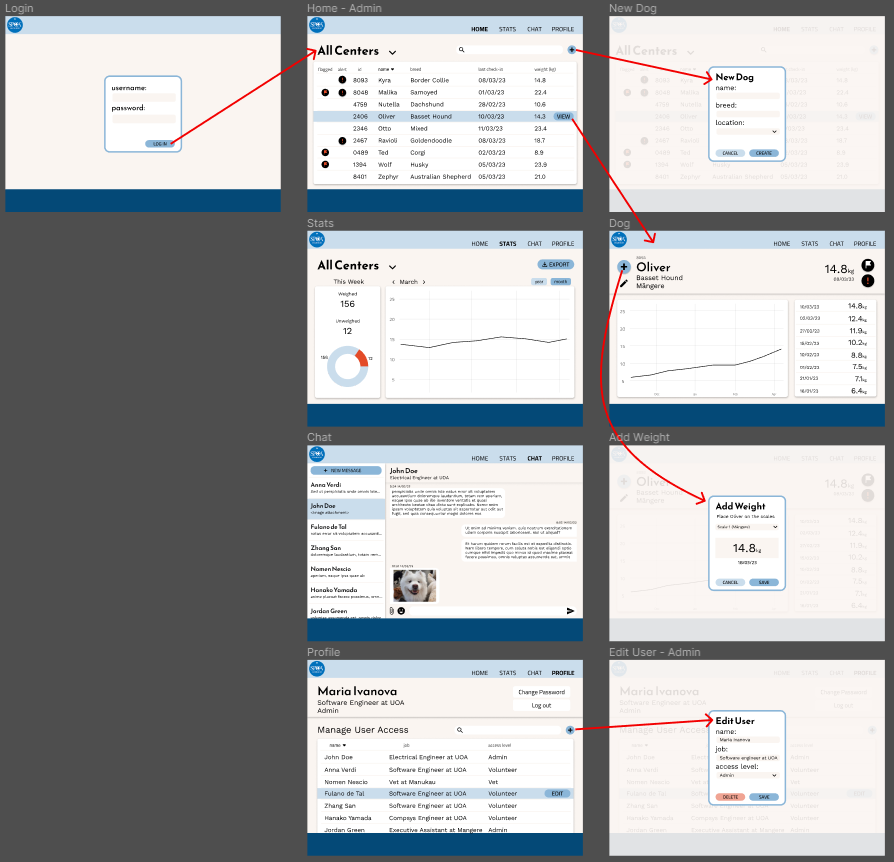
\includegraphics[scale=0.6]{sw-web-app-ui.png}
	\caption{Web App High-fidelity Prototype.}
	\label{fig:webapp-1}
\end{figure}



